\section{Big Data}


A quantidade de informação que está disponível para a humanidade é enorme e a medida que o conhecimento humano se expande, maior é a quantidade dessa informação que precisa ser armazenada e analisada. Além da quantidade, o fluxo e variedade dessas informações constantemente desafiam a indústria e a academia a medida em que a quantidade de \textit{big  data} aumenta exponencialmente. Essa seção apresenta uma definição detalhada de o que é \textit{big data} e as tecnologias que apoiam esse domínio.

\subsection{O que é Big Data?}

Em um estudo divulgado em 2011 o tamanho do universo digital quebrou a barreira dos \textit{zettabytes} e esse número está crescendo rapidamente~\cite{emcuniversedigital}. Cientistas de diversas áreas estão vendo o grande potencial de conhecimento que se pode adiquirir pela análise e armazenamento de informação digital. Conforme já dito anteriormente o conceito de ``grande (\textit{big})''  evoluiu no decorrer da nossa história. Na década de 70, grande significava \emph{kilobytes}; ao longo do tempo cresceu para \emph{gigabytes} e em seguida, a \emph{terabytes}. Atualmente já podemos dizer que grande varia de \emph{petabytes}  até \emph{exabytes}~\cite{WNextBigData}. Contudo  o  conceito de \textit{big data} não se dá somente por tamanho ou domínio, mas também por um conjunto de características que o difere de uma base de dados comum.

Segundo Gartner, empresa líder em pesquisa e consultoria na área de TI, \emph{big data} é definido, em geral, como uma massa de dados de grande volume, velocidade e variedade de informações que exigem formas inovadoras de processamento para maior visibilidade e tomada de decisão~\cite{conceitoGartner}. A maioria dos estudiosos compartilham dessa mesma definição e afirmam que \textit{big data} é caracterizado por no mínimo três V's. Volume, variedade e  velocidade ~\cite{ibmbigdatavvv,fromdbtobigdata}.

Volume é a característica mais fácil de se perceber. Geramos enormes quantidades de dados todos os dias, e essa quantidade só tende a aumentar. Redes sociais, dispositivos móveis que guardam nossas informações, sites que armazenam nossas preferências, dispositivos de busca que indexam as páginas da web e a popularização da computação em nuvem nos colocam em uma época de grande volume de dados, uma época em que tudo é informação, tudo é valioso, tudo pode ser extraído. Cada dia fica mais comum grandes empresas terem de lidar com dados na ordem de \textit{petabytes}. Variedade é outra característica que é de fácil percepção, pois os dados são de diversas naturezas como email, dados gerados por mídias sociais (\textit{blogs}, Twitter, Youtube, Facebook, \textit{Wikis}), documentos eletrônicos, apresentações, fotos, mensagens instantâneas, dados médicos, videos, etc. A característica de velocidade é explicada quando precisamos processar os dados praticamente em tempo real como em controle de tráfego, detecções de fraudes e propagandas dinâmicas na web. Os dados são cada vez mais usados para tomadas de decisão em tempo real~\cite{promiseperil}.

\begin{table}
	\caption{Tabela de bytes}
	\begin{center}
	\begin{tabular}{ccc}
		\hline
			\textbf{Nome} & \textbf{Tamanho} & \textbf{Abreviação} \\
		\hline
			\texttt{Kilobyte}	& $10^3$ & KB \\
			\texttt{Megabyte}	& $10^6$ & MB \\
			\texttt{Gigabyte}	& $10^9$ & GB \\
			\texttt{Terabyte}	& $10^{12}$ & TB \\
			\texttt{Petabyte}	& $10^{15}$ & PB \\
			\texttt{Exabyte}	& $10^{18}$ & EB \\
			\texttt{Zettabyte}	& $10^{21}$ & ZB \\
			\texttt{Yottabyte}	& $10^{24}$ & YB \\
		\hline
	\end {tabular}
	\end{center}
	\label{tab:bytes}
\end{table}

Dada a problemática do armazenamento, ao se deparar com os limites de técnicas e ferramentas disponíveis, o mercado tratou de criar suas próprias soluções de gerenciamento de dados, em sua maioria não relacional. Usando a tecnologia apropriada, profissionais capacitados podem transformar grandes massas de dados em informações muito valiosas. Muitos sistemas comerciais relacionais se dizem capazes de lidar com vários \textit{petabytes} de base de dados (Greenplum, Netezza, Teradata, ou Vertica). Apesar dessa quantidade de dados atender a grande maioria das empresas, existem empresas de grande porte como o Google e o Facebook que não são atendidas e precisaram criar suas próprias soluções, além disso, sistemas \textit{open source} como Postgres  não tem o mesmo nível de escalabilidade que os comerciais ~\cite{fromdbtobigdata}.

\subsection{Bases de dados relacionais}

Quando pensamos em armazenamento de dados em SGBDs logo associamos essa ideia ao método tradicional que inclui bancos de dados como MySQL, PostgreSQL, modelagem relacional e esquemas de dados bem definidos. O modelo de dados relacional foi introduzido por Edgar F. Codd, da IBM Research, em 1970, em um artigo que conseguiu atrair grande atenção devido à simplicidade e base matemática. Os SGBDs relacionais mais populares atualmente são DB2 e Informix Dynamic Server (IBM), Oracle e Rdb (Oracle), Sybase SGBD (Sybase) e SQLServer e Access (Microsoft). Ainda temos os de código aberto como o MySQL e PostgreSQL.

O modelo relacional representa o banco de dados como uma coleção de relações. Uma relação é similar a uma tabela de valores ou um arquivo de registros. Cada tabela é formada por uma ou mais colunas de dados. Por sua vez, cada linha na tabela contém uma instância única de dado para as categorias de colunas definidas. No modelo relacional é possível criar conexões entre as tabelas e os  campos e os formatos dos valores são bem definidos, ou seja, possui um \textit{schema} de dados~\cite{SBElmasri,nosqlliveup}. Na Figura \ref{fig:modelorelacional} temos o modelo de dados relacional implementado no protótipo que foi utilizado para a realização dos testes.

	\begin{figure}[!htbp]
		\begin{center}
			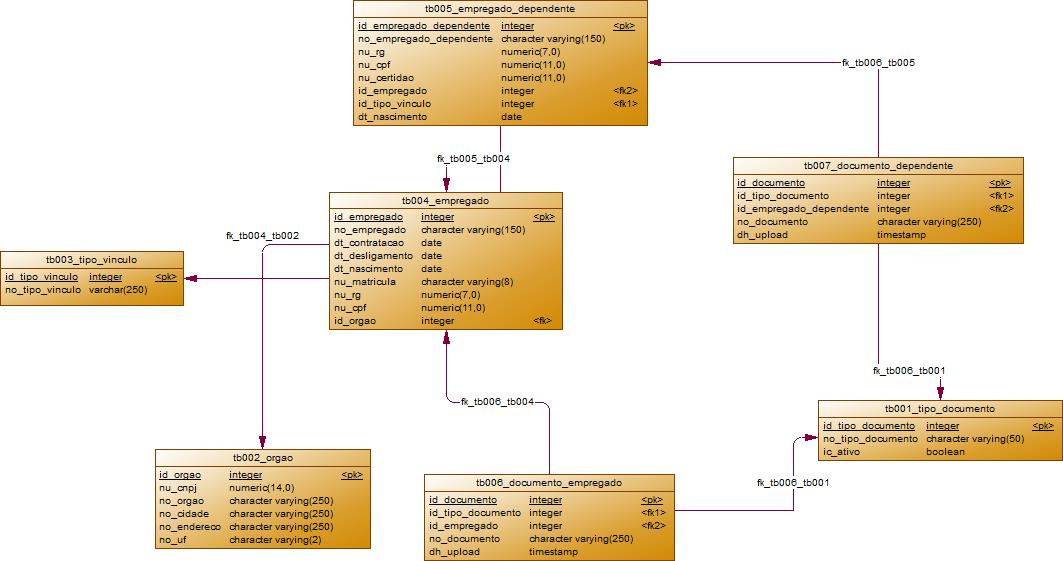
\includegraphics[width=1\textwidth]{modelo_relacional}
		\end{center}
		\caption{Modelo Relacional }
		\label{fig:modelorelacional}
	\end{figure}

Umas das características mais importantes das bases de dados relacionais são as garantias das propriedades ACID  ~\cite{Orendanalysisand}. ACID é um acrônimo para \textit{Atomicity}(Atomicidade), \textit{Consistency}(Consitência), \textit{Isolation} (Isolamento) e \textit{Durability} (Durabilidade).
Atomicidade significa que todas as etapas de uma transação serão executadas, caso contrário a transação será abortada sem interferir no banco de dados. Consistência significa que um banco de dados estará em um estado consistente antes e após cada transação. Caso as mudanças de uma transação violarem a regra de consistência, então todas as mudanças serão revogadas para garantir que somente os dados realmente válidos serão escritos no banco de dados. Isolamento, por sua vez, significa que as transações não podem visualizar as mudanças que não foram submetidas ao banco. Como as alterações que resultaram em erros. Finalmente, a propriedade de durabilidade requer que os dados sejam escritos no banco antes da transação ser confirmada. Caso haja uma falha de energia os dados não serão perdidos.

Os SGBDs (Sistemas Gerenciadores de Banco de Dados) relacionais proveem diversas garantias aos seus usuários, como validação, verificação e garantias de integridade dos dados, controle de concorrência, recuperação de falhas,  entre outros. Todas essas características mantém os SGBDs como principal solução na maioria dos ambientes computacionais, mas não impediram o surgimento de problemas, em alguns casos, causados pela rígida estrutura definida pelo \textit{layout} das tabelas, nomes e tipos das colunas.

As abordagens mais usadas para manipular grandes bases nesse tipo de estrutura são os \textit{data warehouses} e \textit{data marts}. Um \textit{data warehouse} é um banco de dados relacional usado para armazenar, analisar e gerar relatórios sobre os dados. O \textit{data mart} é a camada usada para acessar o \textit{data warehouse}. As duas abordagens usadas para se armazenar dados em um \textit{data warehouse} são a normalização e a modelagem dimensional~\cite{bigdataarchitectureandapproach}.

Por outro lado, com a evolução das aplicações e com requisitos cada vez mais exigentes, foram surgindo casos em que os bancos de dados relacionais não escalavam. Operações de \textit{joins} estão presentes nos menores dos bancos de dados relacionais, e esse tipo de operação é lenta. Para que SGBDs relacionais consigam garantir consistência para os dados eles usam o conceito de transações, o que requer um bloqueio nos dados durante um certo período de tempo.  Dessa forma, quando o banco recebe várias requisições simultâneas em um mesmo dado os usuários são obrigados a esperarem em uma fila~\cite{cassandraguide}.

A necessidade de transformar os dados em tabelas causa um aumento na complexidade da operação, pois requer o uso de complexos algoritmos de mapeamento e estrutura. Mesmo quando uma base de dados pode ser coberta pelo modelo relacional, às vezes as diversas garantias providas por esse modelo gera uma sobrecarga que não seria necessária para tarefas simples. O \textit{schema} rigoroso pode ser pesado para aplicações que precisam de velocidade, como aplicações web e \textit{blogs} que possuem diversos tipos de atributos. Textos, comentários, imagens, vídeos, código fonte e outras informações precisam ser armazenadas em diversas tabelas, e como as aplicações na web são muito ágeis, precisam ser amparadas por uma base de dados igualmente ágil e com um \textit{schema} de fácil adaptação ~\cite{nosqlevaluation}.

O grande aumento na quantidade de dados deve ser considerado por grandes empresas como Facebook, Amazon e Google. Além de tratar \textit{terabytes}/\textit{petabytes} de dados, realizar requisições de leitura e escrita na base a todo o momento essas empresas devem se preocupar com o tempo que essas transações estão levando, ou seja, a latência. Para tratar esses requisitos é preciso manter milhares de máquinas com um \textit{hardware} moderno e veloz. Por ter que cumprir com os requisitos de ACID e manter os dados normalizados, um modelo relacional não é adequado para esse cenário, visto que as operações de \textit{join} bloqueiam os dados e influenciam negativamente no desempenho da aplicação.

Outro requisito fundamental para as grandes empresas é a disponibilidade de seus serviços. Para isso a base de dados deve ser facilmente replicável e fornecer uma forma automática de tratamento à falha de bases ou do \textit{datacenter}. Esses SGBDs também devem ser capazes de balancear a carga em várias máquinas para não sobrecarregar um único servidor. Bancos relacionais priorizam a consistência em detrimento à disponibilidade e também possuem um mecanismo de replicação limitado.

Esses problemas podem ser resolvidos de algumas formas. Primeiramente se opta por um \textit{upgrade} simples de \textit{hardware}. Se o problema persistir a próxima opção seria adicionar novos servidores ao \textit{cluster}, porém com os problemas de consistência e replicação durante o uso regular e em cenários de falha. A próxima etapa seria melhorar a configuração do gerenciador de banco de dados. Caso as opções de melhoria no SGBD se esgotem é preciso melhorar a aplicação. Verifica-se o desempenho das consultas, cria-se índices e etc. Se o desempenho ainda não for satisfatório então talvez seja necessário colocar uma camada de \textit{cache}, mas que também gera um problema de consistência. Se mesmo assim o desempenho não atender as expectativas, então é necessário pensar novamente no SGBD. A última opção seria uma desnormarlização do banco, mas assim se estaria indo contra os princípios da modelagem relacional e das regras normais~\cite{cassandraguide}.

Dado toda essa problemática surge uma opção. Bancos de dados que não seguem o paradigma relacional. Os dados não são normalizados.

\subsection{Bases Não Relacionais}

O NoSQL foi proposto em 2009 e quebrou os limites das bases de dados relacionais e das propriedades ACID. Os bancos de dados NoSQL geralmente não proveem as propriedades ACID: atualizações são eventualmente propagadas, mas há garantias limitadas para a consistência de leituras. Alguns autores sugeriram  o acrônimo ‘BASE’ em contraste ao ‘ACID’ ~\cite{scalablesqlandnosql}. O teorema CAP, o teorema BASE e o conceito de consistência eventual são os fundamentos do NoSQL, discutidos no decorrer dessa seção.

\subsubsection{Teorema CAP}

O teorema CAP (Figura \ref{fig:captheorem}) foi proposto por Eric Brewer. CAP significa Consistência,  disponibilidade e tolerância a particionamento de rede.  A idéia principal desse teorema é que os sistemas distribuídos não podem atender, ao mesmo tempo, essas três características. Podem atender somente duas delas ~\cite{nosqlaplicassandra}.

	\begin{figure}[!htbp]
		\begin{center}
			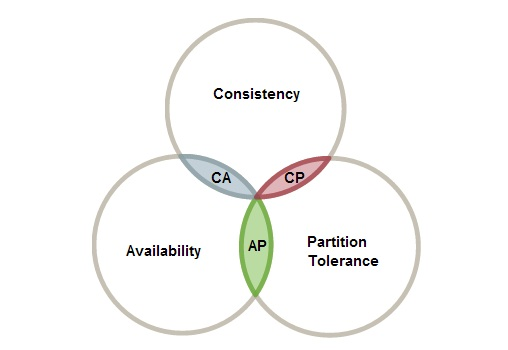
\includegraphics[width=0.8\textwidth]{captheorem}
		\end{center}
		\caption{Teorema CAP ~\cite{capimage} }
		\label{fig:captheorem}
	\end{figure}

Nesse caso a disponibilidade permite que os clientes sempre possam executar leituras e escritas em um certo período de tempo. Um banco de dados distribuído que permite particionamento é tolerante à falhas de conexão e permite a distribuição em nós separados ~\cite{Orendanalysisand}.

Um sistema que permite o particionamento só poderá prover uma consistência forte se sacrificar a disponibilidade. Isso porque cada operação de escrita somente será concluída se os dados forem replicados para todos os nós, o que nem sempre é possível em um ambiente com falhas de conexão ou outras falhas de \textit{hardware} ~\cite{Orendanalysisand}.

Sendo assim, temos três arquiteturas possíveis: CA, AP e CP. Como atualmente a grande maioria dos sistemas é implantada na web, a disponibilidade é indispensável. Isso nos permite utilizar somente com as arquiteturas CA e AP. Para sistemas web, a disponibilidade e a tolerância ao particionamento são mais importantes que a consistência. Já é suficiente quando um sistema web possui consistência eventual ~\cite{nosqlaplicassandra}.

\subsubsection{Teorema BASE}

O teorema BASE é um produto do teorema CAP. As propriedades BASE são completamente diferentes das ACID. BASE é um acrônimo para: \textit{Basically Available} (Basicamente Disponível), \textit{Soft-state}(base otimizada pelo uso) e \textit{Eventual consistency} (Disponibilidade Eventual) ~\cite{nosqlaplicassandra}.

\begin{itemize}
\item \textit{BasicallyAvailable} : Significa que eventuais falhas de particionamento são suportadas.
\item \textit{Soft-state}: Significa que em um período de tempo o estado do sistema pode ser assíncrono.
\item \textit{Eventual consistency}: O sistema ‘deve’ ser consistente.
\end{itemize}

\subsubsection{Consistência Eventual}

Por causa do teorema CAP, a maioria dos banco de dados NoSQL proveem consistência eventual. Abaixo estão as definições de consistência forte e consistência eventual.

Consistência forte: Significa que todos os processos conectados em um banco de dados sempre verão a mesma versão de um valor e uma nova atualização é instantaneamente refletida por qualquer operação de leitura até outra mudança ser feita por outra operação de escrita ~\cite{Orendanalysisand}. Na Figura \ref{fig:strongconsistency} temos um exemplo gráfico.

	\begin{figure}[!htbp]
		\begin{center}
			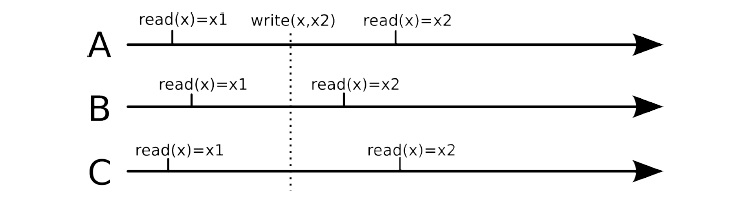
\includegraphics[width=0.8\textwidth]{strongconsistency}
		\end{center}
		\caption{Consistência Forte: O processo A, B e C sempre estão vendo a mesma versão do banco de dados ~\cite{Orendanalysisand}.}
		\label{fig:strongconsistency}
	\end{figure}

Consistência Eventual: É um tipo de consistência fraca. Não garante que todos os processos veem a mesma versão dos dados. Isso pode ocorrer por causa das janelas de inconsistência e é geralmente causada pela replicação dos dados nos diferentes nós ~\cite{Orendanalysisand}. Na Figura \ref{fig:eventualconsistency} temos um exemplo gráfico.

	\begin{figure}[!htbp]
		\begin{center}
			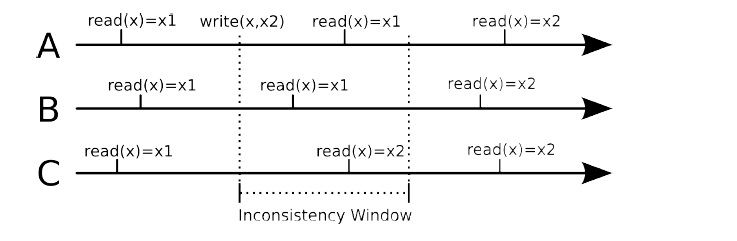
\includegraphics[width=0.8\textwidth]{eventualconsistency}
		\end{center}
		\caption{Consistência Eventual: Os processos A, B e C podem visualizar diferentes versões dos dados durante a janela de inconsistência causada pela replicação assíncrona ~\cite{Orendanalysisand}.}
		\label{fig:eventualconsistency}
	\end{figure}







